\chapter{SUPPLEMENTARY INFORMATION FOR CHAPTER 2} \label{ch:alignpair-supplement}

\clearpage

\section*{Benchmark Results}

\begin{table}[H]
\centering
\begin{tabular}[t]{l|r|r|r|r|r|r}
\hline
  & dseq & Perfect & Best & Imperfect & F1 pos selection & F1 neg selection\\
\hline
tri-MG94 & 0.00221 & 5793 & 5139 & 1048 & 0.98073 & 0.99809\\
\hline
MAFFT & 0.01471 & 5292 & 4692 & 1549 & 0.84314 & 0.98411\\
\hline
PRANK* & 0.01828 & 4725 & 4774 & 2116 & 0.86749 & 0.98698\\
\hline
MACSE & 0.01399 & 2861 & 3737 & 3980 & 0.79456 & 0.98199\\
\hline
Clustal$\Omega$ & 0.02929 & 2893 & 2615 & 3948 & 0.68691 & 0.96938\\
\hline
\multicolumn{7}{l}{\rule{0pt}{1em}\textit{*} PRANK produced 42 empty alignments, calculations are based on 7719 alignments.}\\
\end{tabular}
\caption[COATi Triplet-MG94 Benchmark Results]{Accuracy of COATi codon-triplet-mg, PRANK, MAFFT, Clustal$\Omega$, and MACSE on 7761 simulated sequence pairs. Perfect alignments have the same score as the true alignment, best alignments have lowest $d_{seq}$, and imperfect alignments have a different score than the true alignment when at least one method found a perfect alignment.}
\end{table}\label{table:results-tri-mg}


\begin{table}[H]

\centering
\begin{tabular}[t]{l|r|r|r|r|r|r}
\hline
  & dseq & Perfect & Best & Imperfect & F1 pos selection & F1 neg selection\\
\hline
tri-ECM & 0.00238 & 5689 & 5045 & 1118 & 0.97803 & 0.99779\\
\hline
MAFFT & 0.01451 & 5338 & 4677 & 1469 & 0.86048 & 0.98549\\
\hline
PRANK* & 0.01903 & 4803 & 4851 & 2004 & 0.89250 & 0.98912\\
\hline
MACSE & 0.01352 & 2903 & 3787 & 3904 & 0.82181 & 0.98359\\
\hline
Clustal$\Omega$ & 0.02801 & 2979 & 2624 & 3828 & 0.72337 & 0.97244\\
\hline
\multicolumn{7}{l}{\rule{0pt}{1em}\textit{*} PRANK produced 69 empty alignments, calculations are based on 7692 alignments.}\\
\end{tabular}
\caption[COATi Triplet-ECM Benchmark Results]{Accuracy of COATi codon-triplet-ecm, PRANK, MAFFT, Clustal$\Omega$, and MACSE on 7761 simulated sequence pairs. Perfect alignments have the same score as the true alignment, best alignments have lowest $d_{seq}$, and imperfect alignments have a different score than the true alignment when at least one method found a perfect alignment.}
\label{table:results-tri-ecm}
\end{table}

\begin{table}[H]
\centering
\begin{tabular}[t]{l|r|r|r|r|r|r}
\hline
  & dseq & Perfect & Best & Imperfect & F1 pos selection & F1 neg selection\\
\hline
mar-MG94 & 0.00222 & 5808 & 5220 & 1075 & 0.97671 & 0.99766\\
\hline
MAFFT & 0.01505 & 5301 & 4782 & 1582 & 0.85147 & 0.98455\\
\hline
PRANK* & 0.01974 & 4856 & 5015 & 2027 & 0.89928 & 0.99000\\
\hline
MACSE & 0.01429 & 2855 & 3893 & 4028 & 0.81569 & 0.98349\\
\hline
Clustal$\Omega$ & 0.02870 & 2901 & 2610 & 3982 & 0.72399 & 0.97171\\
\hline
\multicolumn{7}{l}{\rule{0pt}{1em}\textit{*} PRANK produced 60 empty alignments, calculations are based on 7695 alignments.}\\
\end{tabular}
\caption[COATi Marginal-MG94 Benchmark Results]{Accuracy of COATi codon-marginal-mg, PRANK, MAFFT, Clustal$\Omega$, and MACSE on 7755 simulated sequence pairs. Perfect alignments have the same score as the true alignment, best alignments have lowest $d_{seq}$, and imperfect alignments have a different score than the true alignment when at least one method found a perfect alignment.}
\label{table:results-mar-mg}
\end{table}

\begin{table}[H]
\begin{tabular}[t]{l|r|r|r|r|r|r}
\hline
  & dseq & Perfect & Best & Imperfect & F1 pos selection & F1 neg selection\\
\hline
mar-ECM & 0.00229 & 5781 & 5135 & 1081 & 0.97052 & 0.99710\\
\hline
MAFFT & 0.01473 & 5379 & 4813 & 1483 & 0.85011 & 0.98491\\
\hline
PRANK* & 0.01953 & 4830 & 4918 & 2032 & 0.87752 & 0.98790\\
\hline
MACSE & 0.01400 & 2953 & 3893 & 3909 & 0.78977 & 0.98159\\
\hline
Clustal$\Omega$ & 0.02918 & 2892 & 2611 & 3970 & 0.67847 & 0.96785\\
\hline
\multicolumn{7}{l}{\rule{0pt}{1em}\textit{*} PRANK produced 49 empty alignments, calculations are based on 7718 alignments.}\\
\end{tabular}
\caption[COATi Marginal-ECM Benchmark Results]{Accuracy of COATi codon-marginal-ecm, PRANK, MAFFT, Clustal$\Omega$, and MACSE on 7767 simulated sequence pairs. Perfect alignments have the same score as the true alignment, best alignments have lowest $d_{seq}$, and imperfect alignments have a different score than the true alignment when at least one method found a perfect alignment.}
\label{table:results-mar-ecm}
\centering
\end{table}

\begin{table}[H]
\centering
\begin{tabular}[t]{l|r|r|r|r|r|r}
\hline
  & dseq & Perfect & Best & Imperfect & F1 pos selection & F1 neg selection\\
\hline
Trip-MG & 0.00113 & 3501 & 2890 & 309 & 0.99278 & 0.99932\\
\hline
MAFFT & 0.00586 & 3162 & 2704 & 648 & 0.91064 & 0.99137\\
\hline
PRANK & 0.00358 & 2829 & 2673 & 981 & 0.90332 & 0.99084\\
\hline
MACSE & 0.00448 & 2552 & 2434 & 1258 & 0.87234 & 0.98857\\
\hline
Clustal$\Omega$ & 0.02099 & 1772 & 1554 & 2038 & 0.75960 & 0.97686\\
\hline
Trip-MG-gor & 0.00118 & 3463 & 2816 & 347 & 0.98993 & 0.99904\\
\hline
\end{tabular}
\caption[COATi Marginal-MG Benchmark Results with Gorilla as Reference]{Accuracy of COATi codon-triplet-mg, PRANK, MAFFT, Clustal$\Omega$, MACSE, and codon-triplet-mg with gorilla as the reference on 4003 of the 7761 simulated sequence pairs where the gorilla sequence was simulated without early stop codons. Perfect alignments have the same score as the true alignment, best alignments have lowest $d_{seq}$, and imperfect alignments have a different score than the true alignment when at least one method found a perfect alignment.}
\label{table:results-gor-ref}
\end{table}

\newpage

\begin{figure}[!ht]
    \centering
    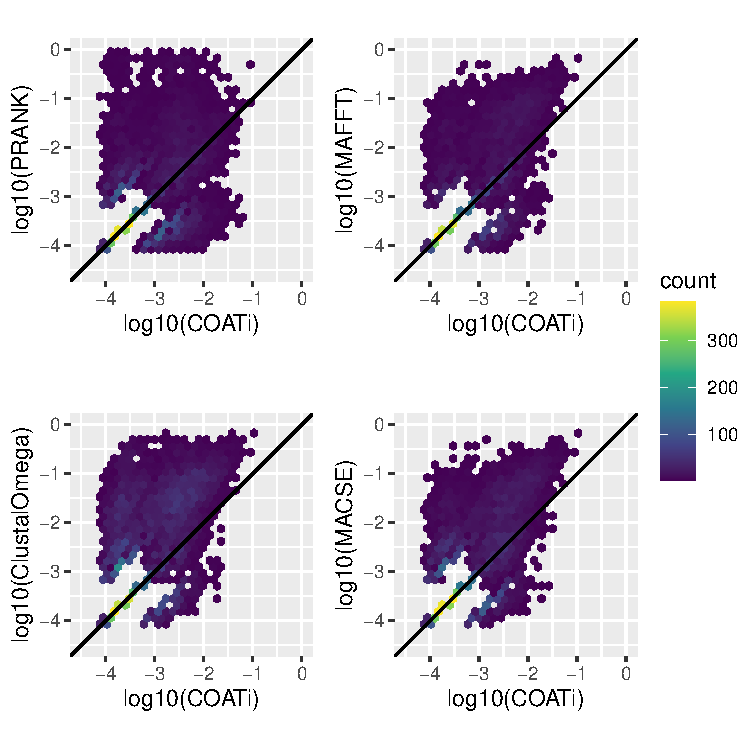
\includegraphics{chapter2/appendix-figures/dseq_plots_tri-mg.pdf}
    \caption[$d_{seq}$ Triplet-MG94]{Comparison of log10-transformed $d_{seq}$ data with pseudocounts between COATi codon-triplet-mg and PRANK, MAFFT, Clustal$\Omega$, and MACSE. COATi was significantly more accurate than other aligners; all p-values were $\leq 1.25e-76$.}
    \label{fig:dseq-tri-mg}
\end{figure}

\begin{figure}[!ht]
    \centering
    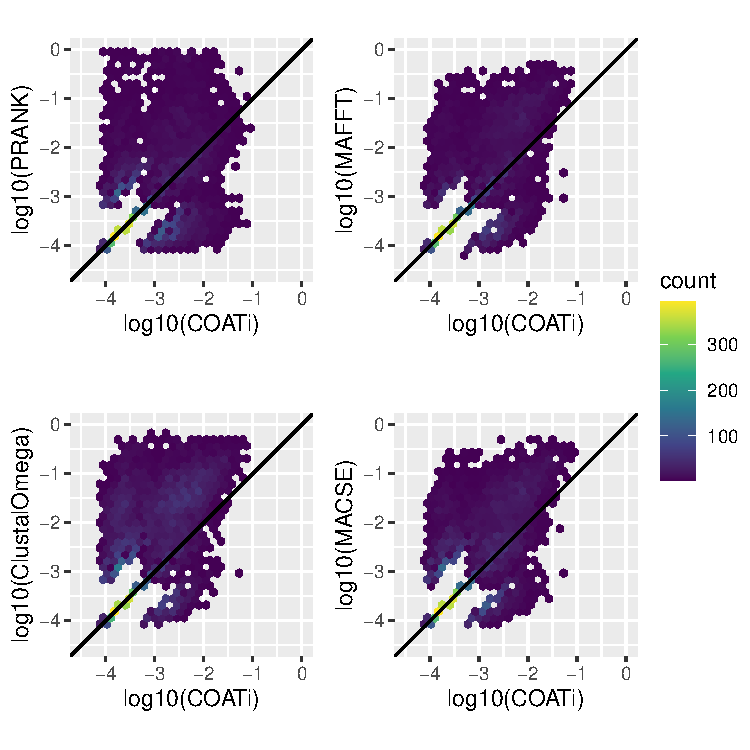
\includegraphics{chapter2/appendix-figures/dseq_plots_tri-ecm.pdf} 
    \caption[$d_{seq}$ Triplet-ECM]{Comparison of log10-transformed $d_{seq}$ data with pseudocounts between COATi codon-triplet-ecm and PRANK, MAFFT, Clustal$\Omega$, and MACSE. COATi was significantly more accurate than other aligners; all p-values were $\leq 3.23e-48$.}
    \label{fig:dseq-tri-ecm} 
\end{figure}

\begin{figure}[!ht]
    \centering
    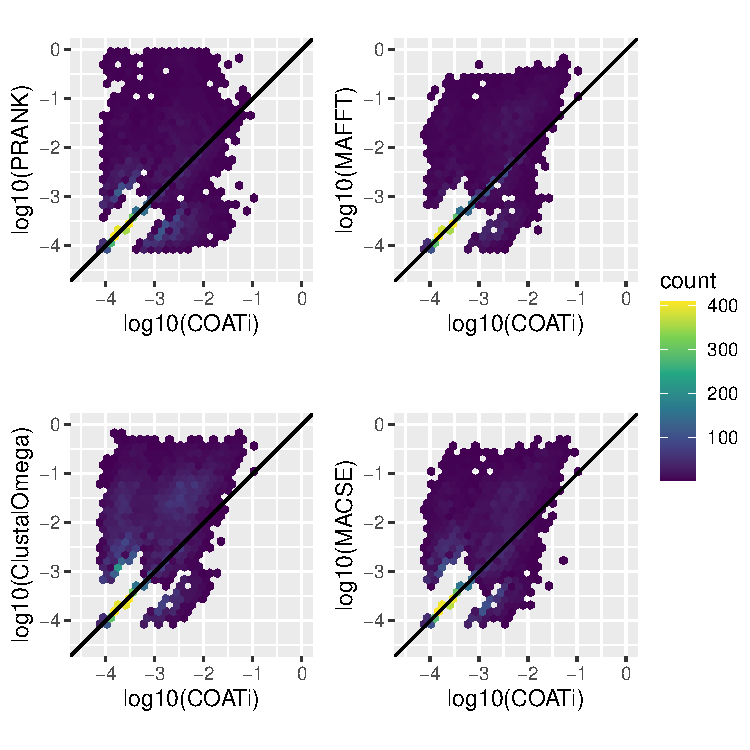
\includegraphics{chapter2/appendix-figures/dseq_plots_mar-mg.pdf} 
    \caption[$d_{seq}$ Marginal-MG94]{Comparison of log10-transformed $d_{seq}$ data with pseudocounts between COATi codon-marginal-mg and PRANK, MAFFT, Clustal$\Omega$, and MACSE. COATi was significantly more accurate than other aligners; all p-values were $\leq 1.99e-53$.}
    \label{fig:dseq-mar-mg}
\end{figure}

\begin{figure}![ht]
    \centering
    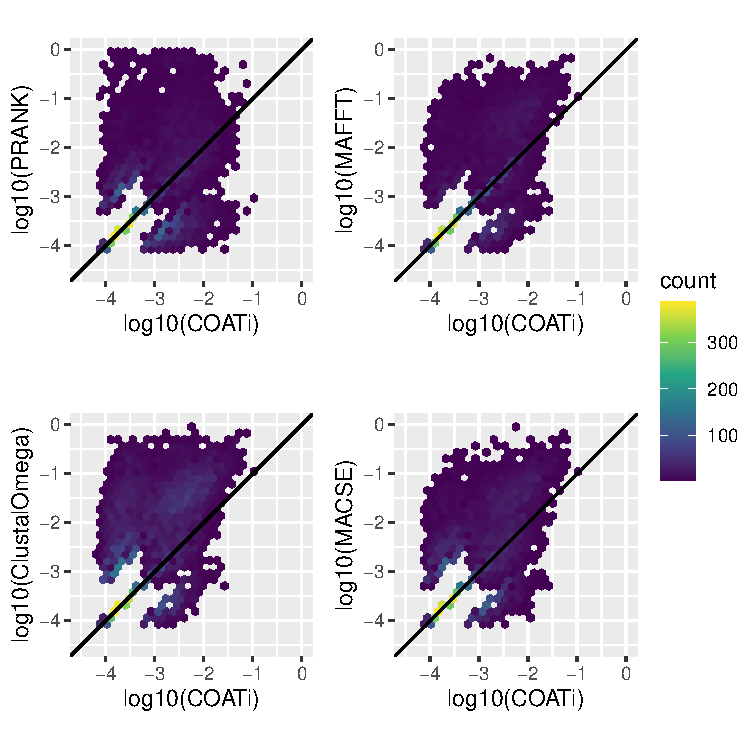
\includegraphics{chapter2/appendix-figures/dseq_plots_mar-ecm.pdf} 
    \caption[$d_{seq}$ Marginal-ECM]{Comparison of log10-transformed $d_{seq}$ data with pseudocounts between COATi codon-marginal-ecm and PRANK, MAFFT, Clustal$\Omega$, and MACSE. COATi was significantly more accurate than other aligners; all p-values were $\leq 1.44e-52$.}
    \label{fig:dseq-mar-ecm}
\end{figure}

\clearpage

% \section{Supplementary Methods} \label{supplementary-methods}

% Ks and Ka represent the number of substitutions per synonymous and
% non-synonymous sites. The ratio of nonsynonymous (Ka) to synonymous (Ks)
% nucleotide substitution rates indicates the selective pressures acting
% on genes. If the ratio is significantly greater than 1, it suggests
% positive selective pressure, meaning that nonsynonymous substitutions
% occur more frequently than synonymous substitutions. A ratio around 1
% can indicate either neutral evolution at the protein level or a mixture
% of positive and negative selective pressures. If the ratio is less than
% 1, it indicates a pressure to maintain protein sequence, known as
% purifying selection. Ks and Ka are calculated using the R package seqinr
% v.4.2-30 \citep{seqinr}.

